% ****** Start of file apssamp.tex ******
%
%   This file is part of the APS files in the REVTeX 4.1 distribution.
%   Version 4.1r of REVTeX, August 2010
%
%   Copyright (c) 2009, 2010 The American Physical Society.
%
%   See the REVTeX 4 README file for restrictions and more information.
%
% TeX'ing this file requires that you have AMS-LaTeX 2.0 installed
% as well as the rest of the prerequisites for REVTeX 4.1
%
% See the REVTeX 4 README file
% It also requires running BibTeX. The commands are as follows:
%
%  1)  latex apssamp.tex
%  2)  bibtex apssamp
%  3)  latex apssamp.tex
%  4)  latex apssamp.tex
%
\documentclass[%
% reprint,
%superscriptaddress,
%groupedaddress,
%unsortedaddress,
%runinaddress,
%frontmatterverbose, 
preprint,
%showpacs,preprintnumbers,
%nofootinbib,
%nobibnotes,
%bibnotes,
 amsmath,amssymb,
 aps,
%pra,
%prb,
%rmp,
%prstab,
%prstper,
%floatfix,
]{revtex4-1}

\usepackage{graphicx}% Include figure files
\usepackage{dcolumn}% Align table columns on decimal point
\usepackage{bm}% bold math
%\usepackage{hyperref}% add hypertext capabilities
%\usepackage[mathlines]{lineno}% Enable numbering of text and display math
%\linenumbers\relax % Commence numbering lines

%\usepackage[showframe,%Uncomment any one of the following lines to test 
%%scale=0.7, marginratio={1:1, 2:3}, ignoreall,% default settings
%%text={7in,10in},centering,
%%margin=1.5in,
%%total={6.5in,8.75in}, top=1.2in, left=0.9in, includefoot,
%%height=10in,a5paper,hmargin={3cm,0.8in},
%]{geometry}

\begin{document}

%\preprint{APS/123-QED}

\title{Proposal for Two Particle Correlation Analyses with BELLE Data}% Force line breaks with \\
%\thanks{A footnote to the article title}%

\author{Yen-Jie Lee}
% \altaffiliation[Also at ]{Physics Department, XYZ University.}%Lines break automatically or can be forced with \\
 \email{yenjie@mit.edu}
\author{Gian Michele Innocenti}%
 \email{ginnocen@mit.edu }
\author{Bibek Pandit}%
\author{Anthony Badea}%
 \affiliation{Massachusetts Institute of Technology}%

%\collaboration{BELLE Collaboration}%\noaffiliation

\date{\today}% It is always \today, today,
             %  but any date may be explicitly specified

\begin{abstract}

\end{abstract}

\pacs{Valid PACS appear here}% PACS, the Physics and Astronomy
                             % Classification Scheme.
%\keywords{Suggested keywords}%Use showkeys class option if keyword
                              %display desired
\maketitle

%\tableofcontents

\section{Introduction}

Two-particle correlations in high-energy collisions provide valuable information for characterizing Quantum Chromodynamics and have been studied previously for a broad range of collision energies in proton-proton (pp), proton-nucleus (pA), and nucleus-nucleus (AA) collisions. Such measurements can elucidate the underlying mechanism of particle production and reveal possible collective effects resulting from the high particle densities accessible in these collisions.

Studies of two-particle angular correlations are typically performed using two-dimentional $\Delta\eta-\Delta\phi$ correlation functions, where $\Delta\phi$ is the difference in the azimuthal angle $\phi$ between the two particles and $\Delta\eta$ is the difference in pseudorapidity $\eta = -\ln(\tan(\theta/2))$. The polar angle $\theta$ is defined relative to the counterclockwise beam direction.

Of particular interest in studies of collective effects is the long-range (large |$\delta\eta$|) structure of the two-particle correlation functions. In this region, the function is less susceptible to known sources of correlations such as resonance decays and fragmentation function of energetic jets. Measurements in high-energy AA collisions have shown significant modification of the long-range structure compared with minimum-bias pp collisions, over a very wide range of collision energies. This long-range correlations are commonly interpreted as a consequence of the hydrodynamical flow of the produced strongly interacting medium and usually characterized by the Fourier components of the azimuthal particle distributions. The extraction of the second and third Fourier components is of great interest because it is closely related to initial collision geometry and its fluctuation. Those measurements allows the extraction of the fundamental transport properties of the medium using hydrodynamic models.

Recently, measurements in pp collisions and pPb collisions have revealed the emergence of long-range, near-side ($\Delta\phi\sim 0$) correlations in the selection of collisions with very high number of final state particles. This ``ridge-like'' correlation has inspired a large variety of theoretical models. Moreover, it was found that the elliptic flow signal exists also in the lowest energy AA collisions at the Relativistic Heavy Ion Collider. 

\subsection{Two-Particle Correlation Function}

\subsection{Preliminary Results from BELLE Open Data}

\section{Summary}



\begin{figure}[!htb]
\begin{center}
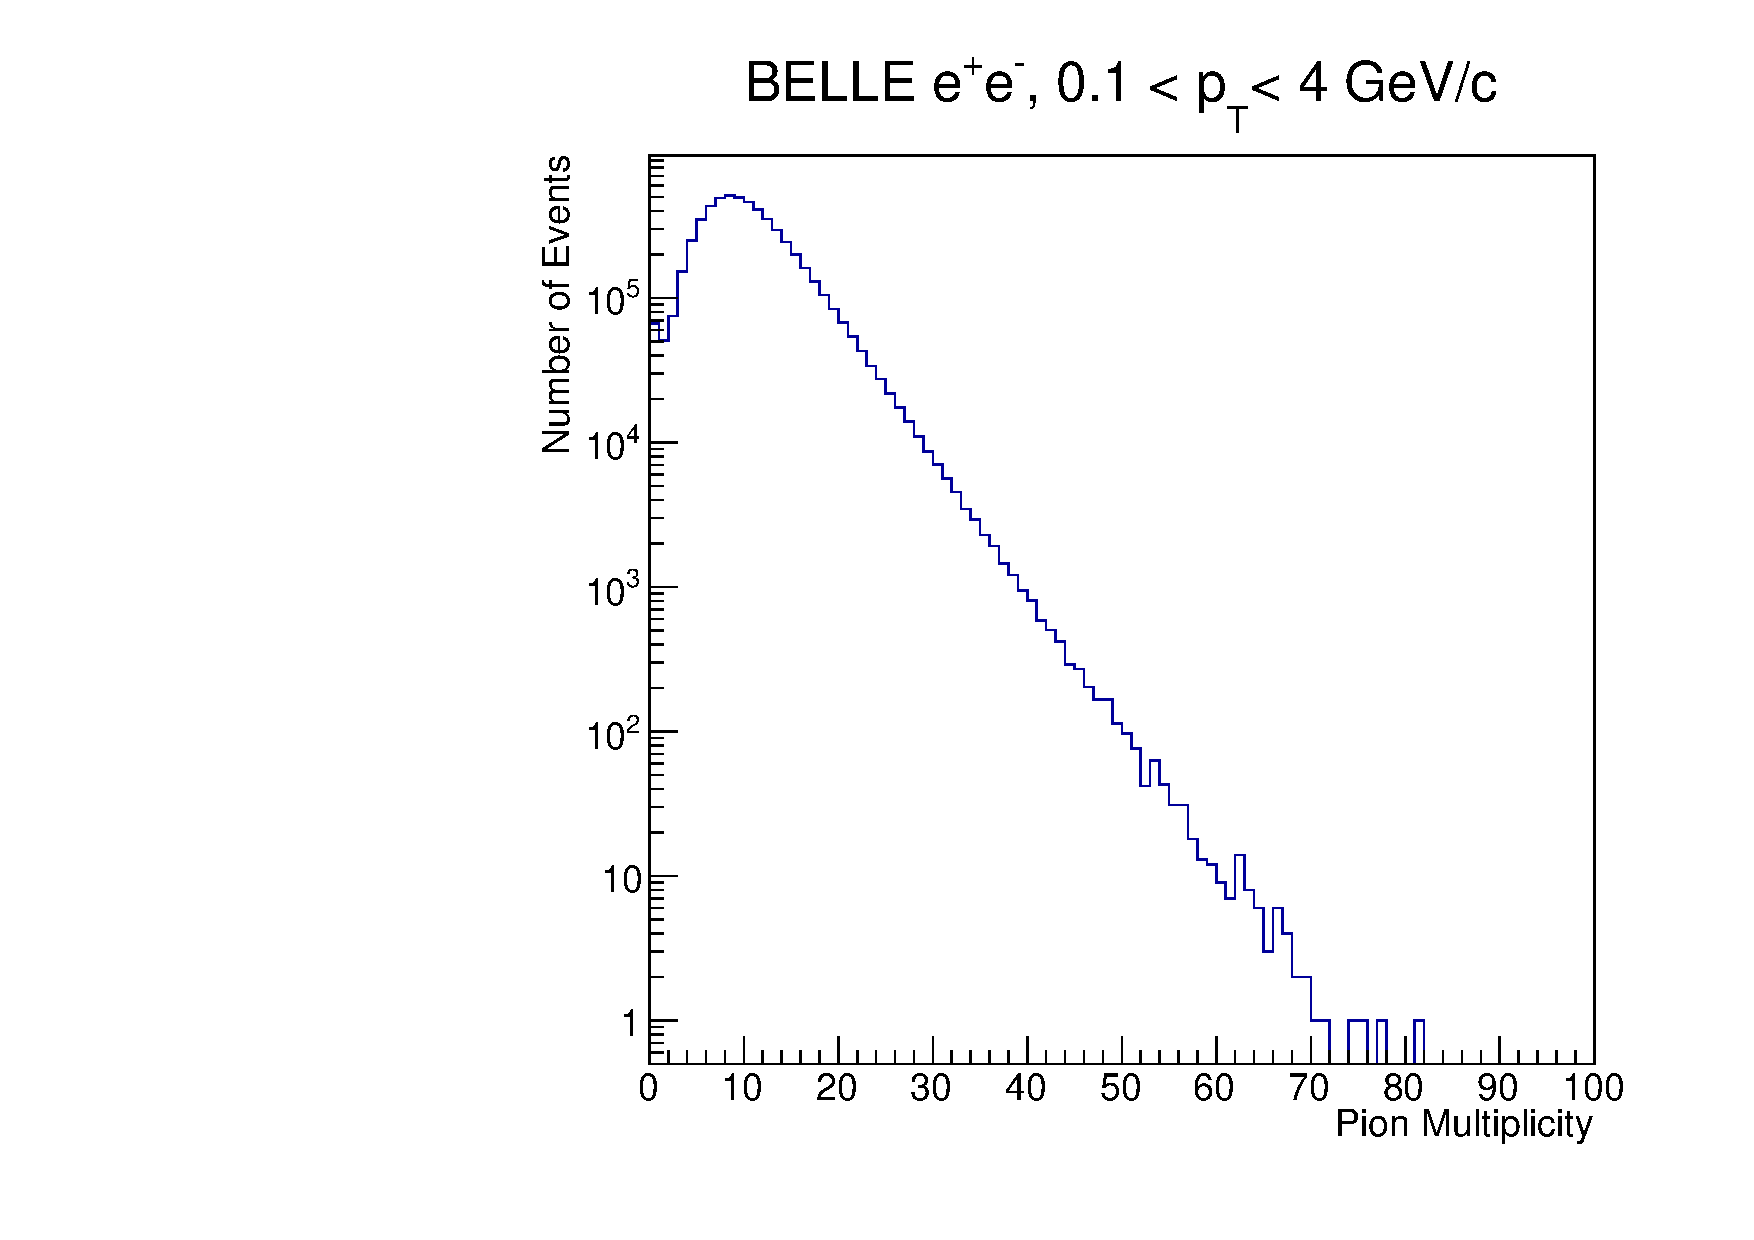
\includegraphics[width=.45\textwidth]{figures/pion_mult.pdf}
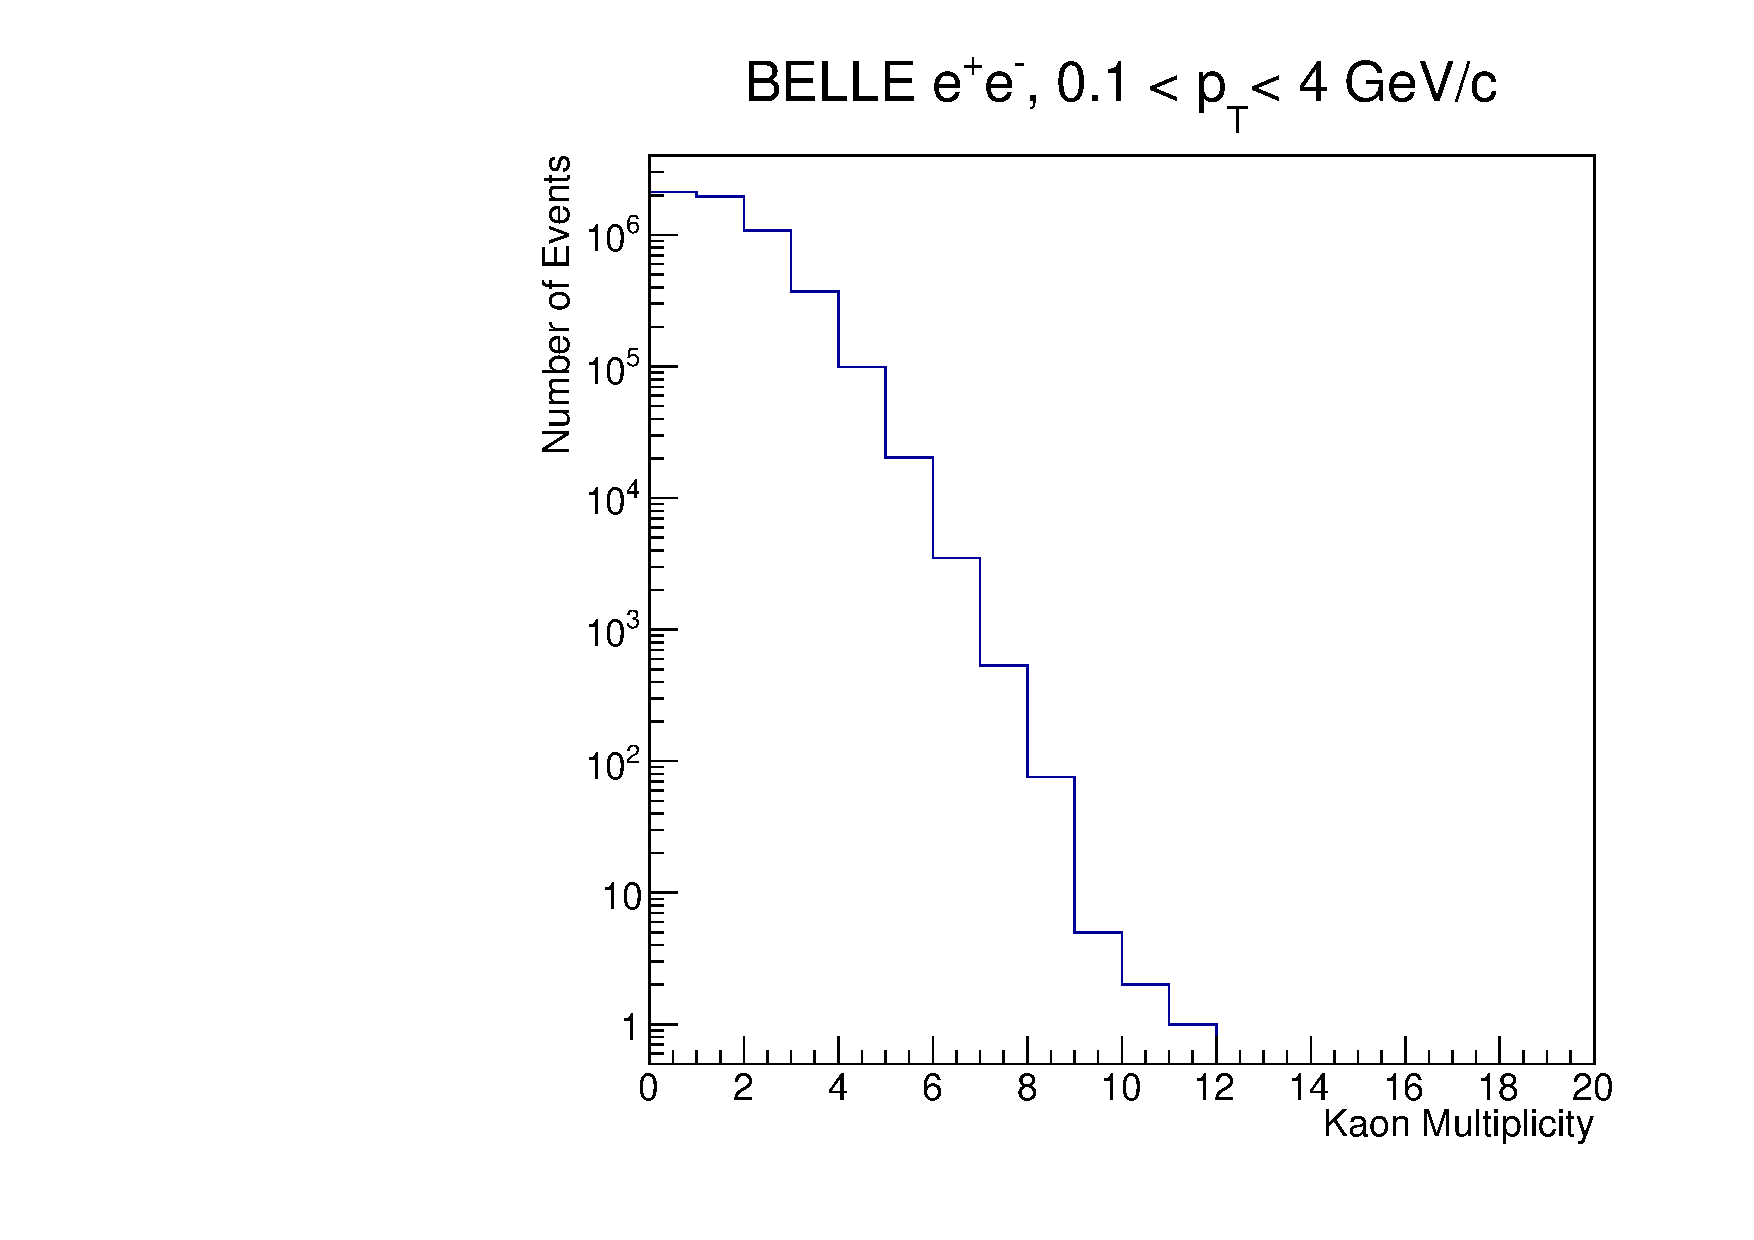
\includegraphics[width=.45\textwidth]{figures/kaon_mult.pdf}
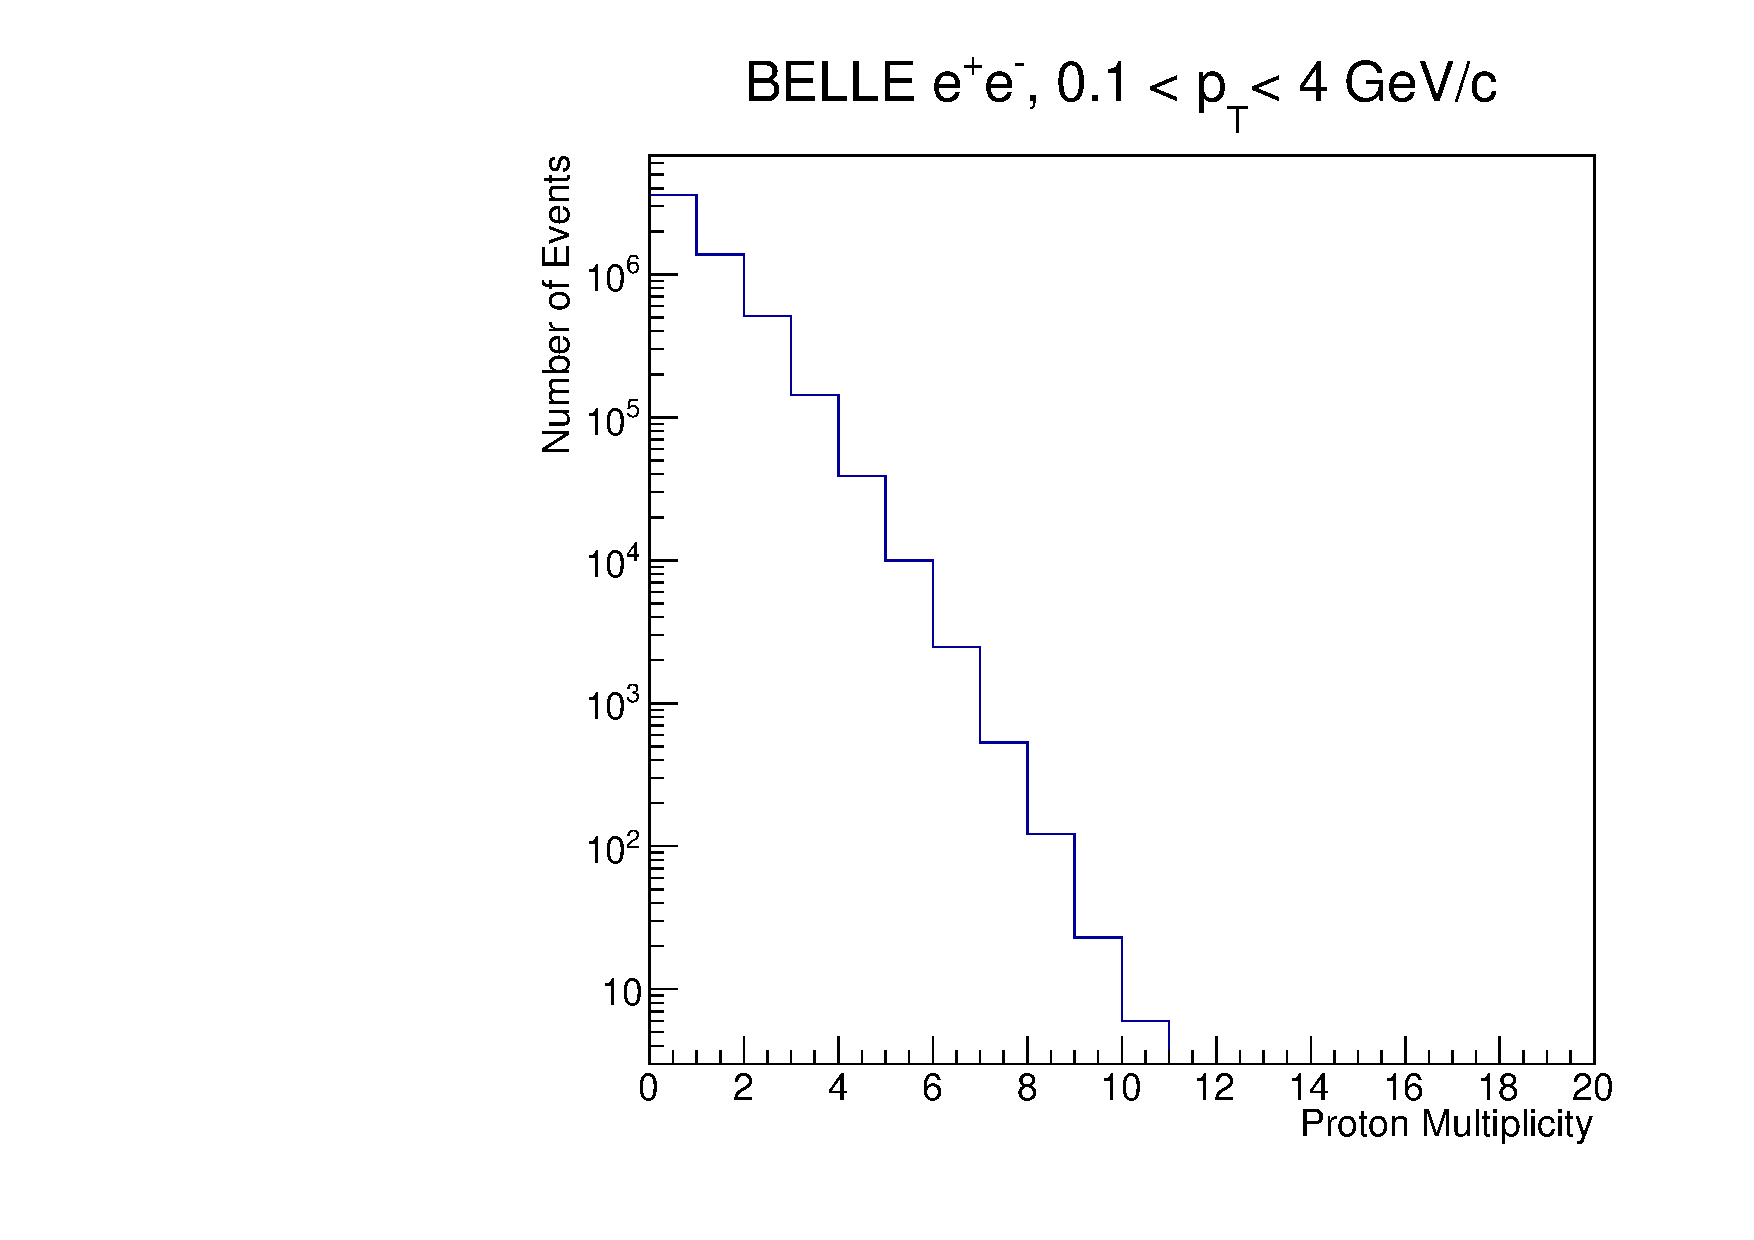
\includegraphics[width=.45\textwidth]{figures/proton_mult.pdf}
\caption{Multipicity of pions (left), kaons (middle), protons (right) }
\label{fig:ridgeBelle} 
\end{center}
\end{figure}

\begin{figure}[!htb]
\begin{center}
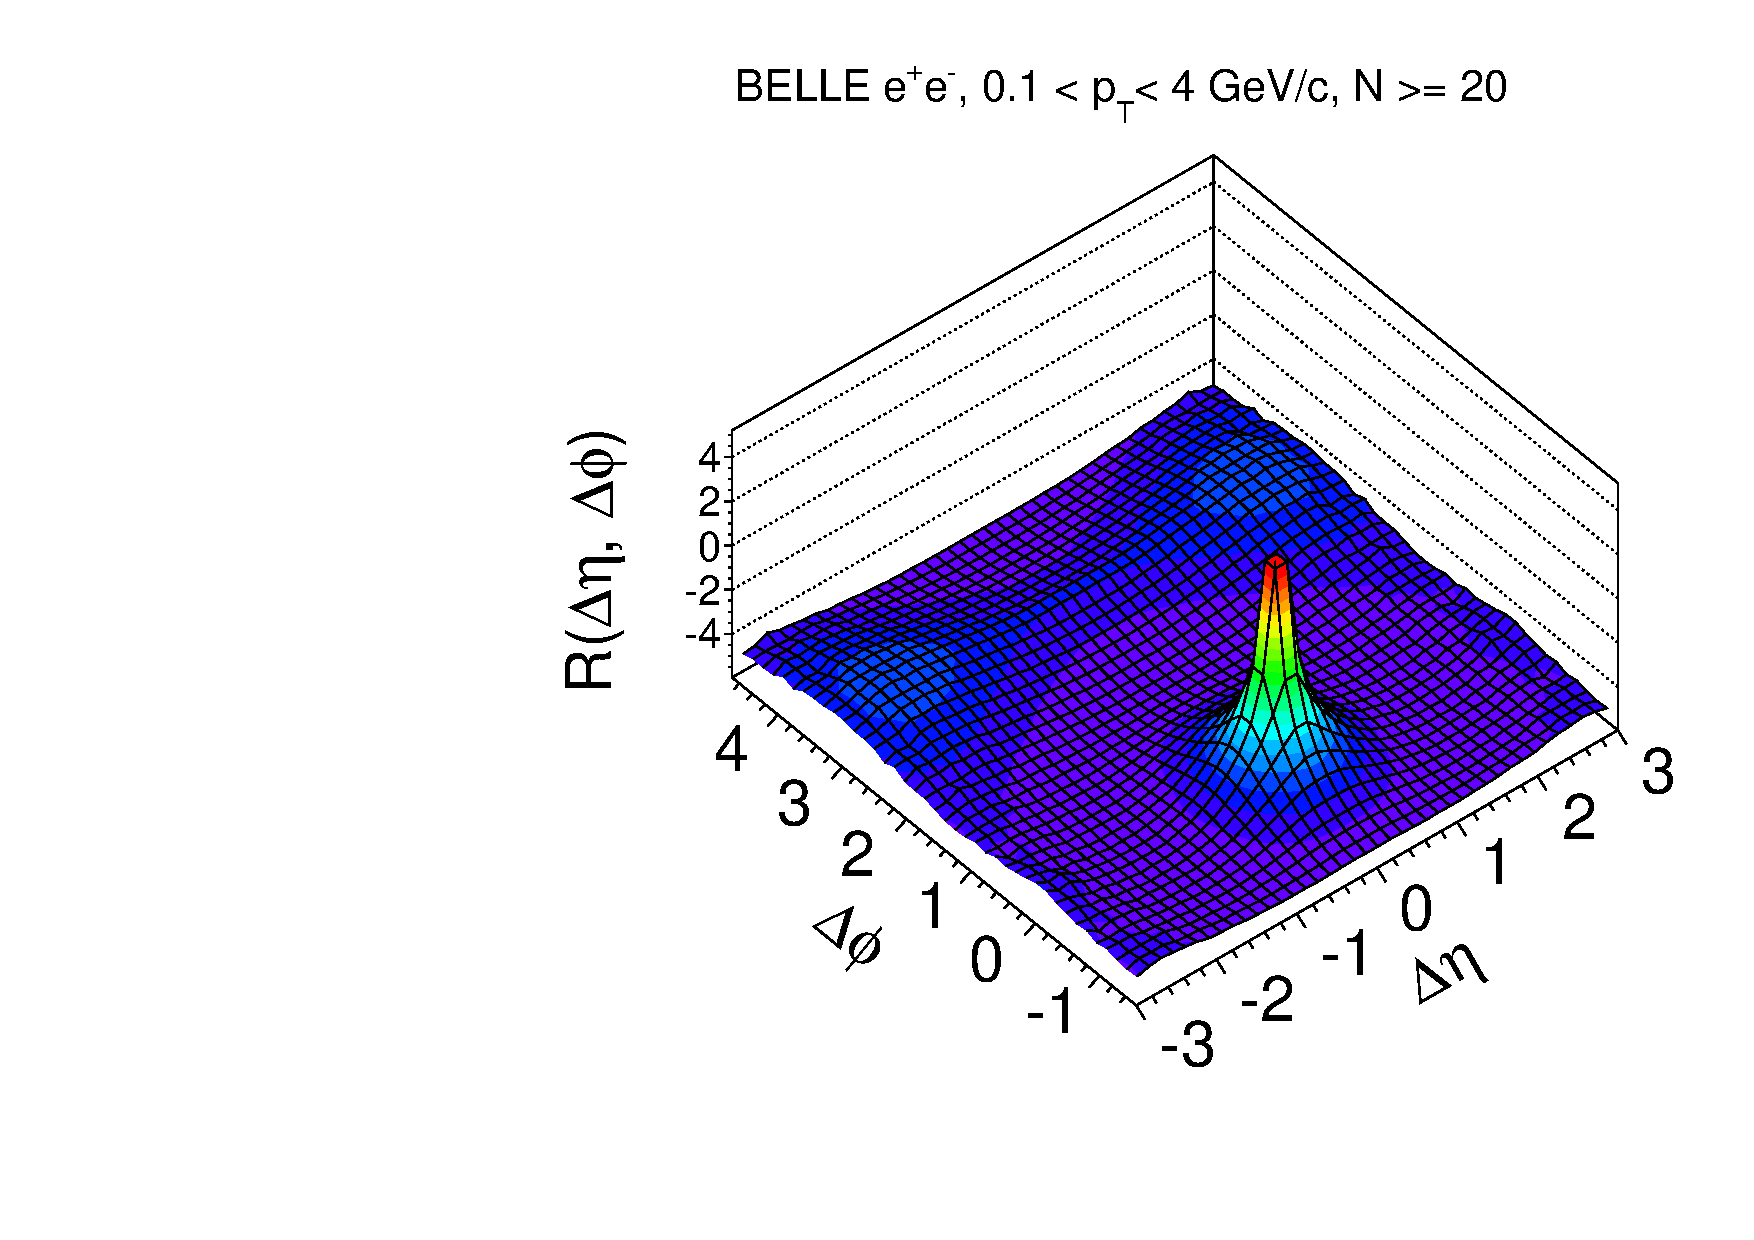
\includegraphics[width=.45\textwidth]{figures/canvasRidgeBelleMult20CutHigh0.pdf}
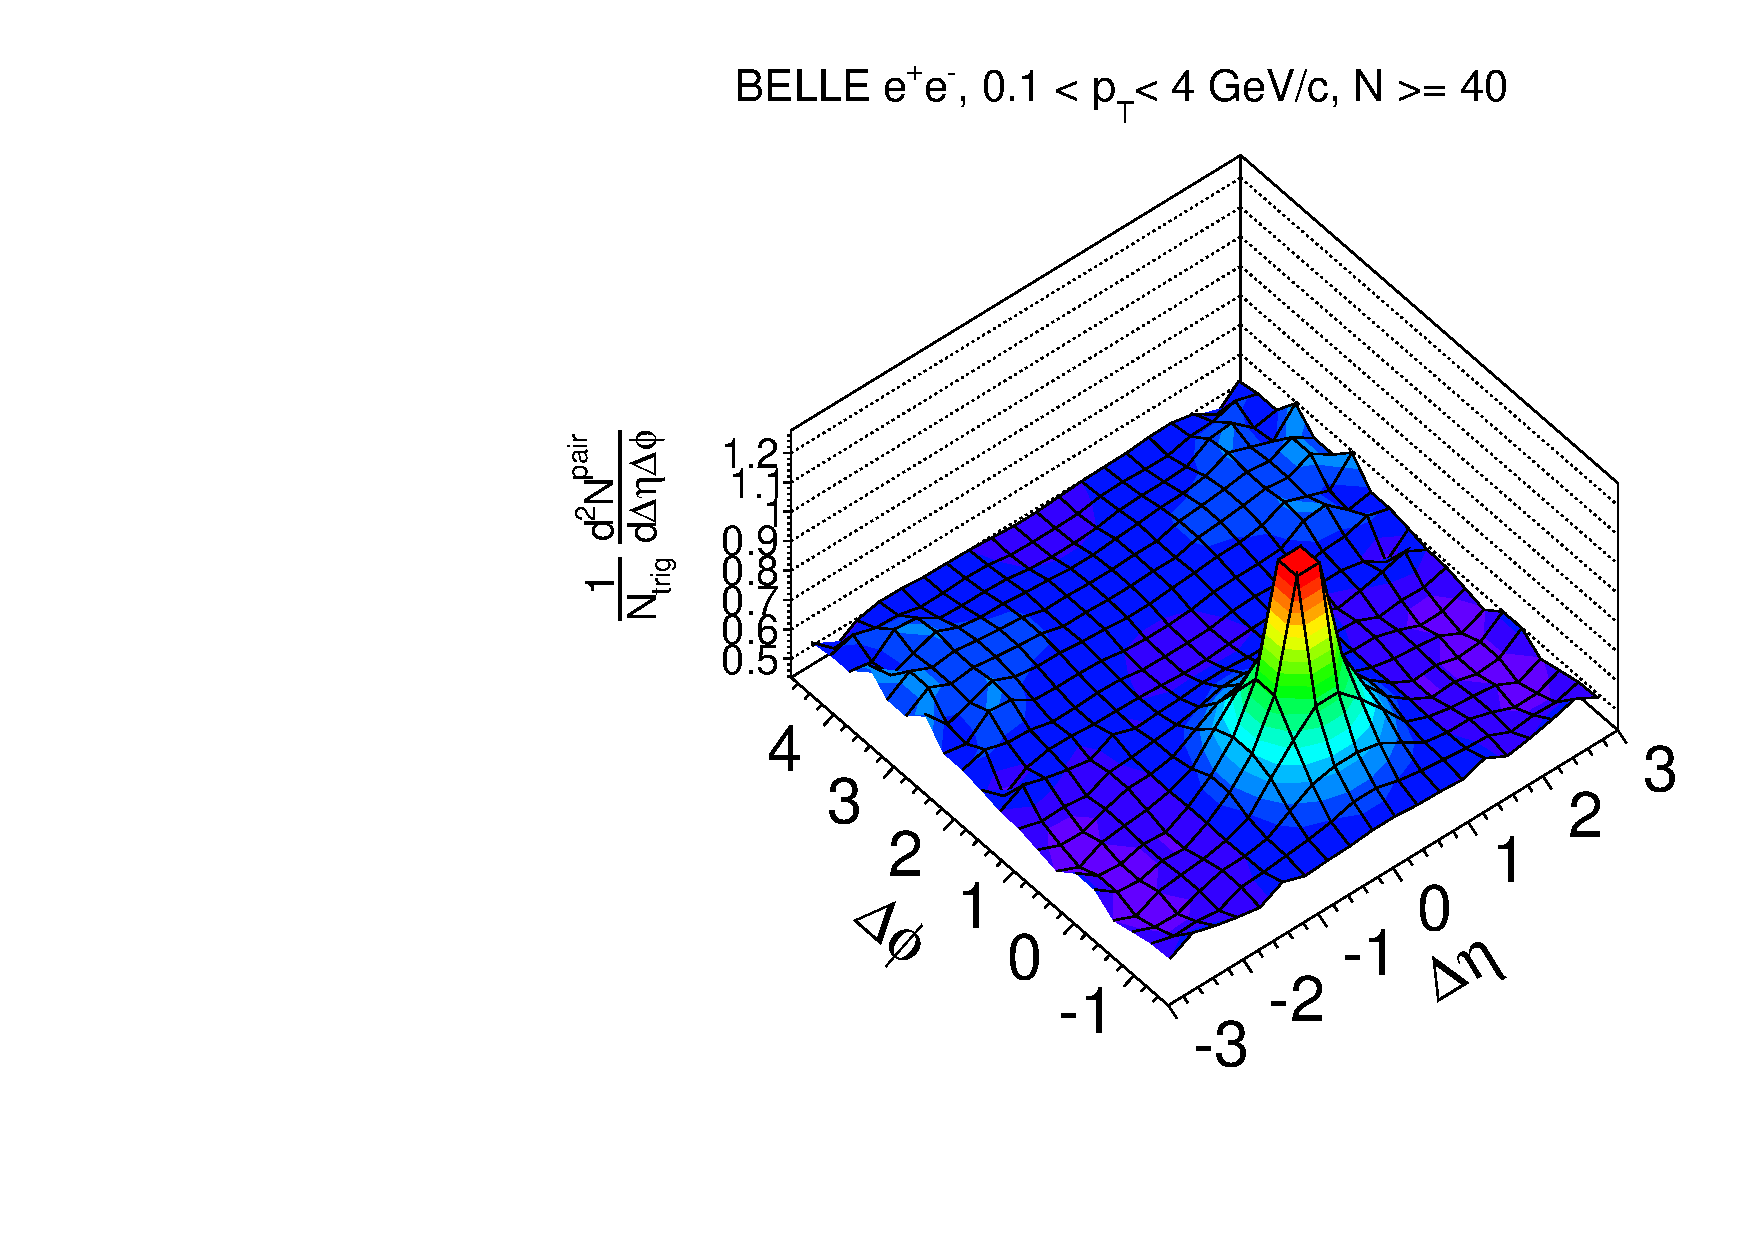
\includegraphics[width=.45\textwidth]{figures/canvasRidgeBelleMult40CutHigh0.pdf}
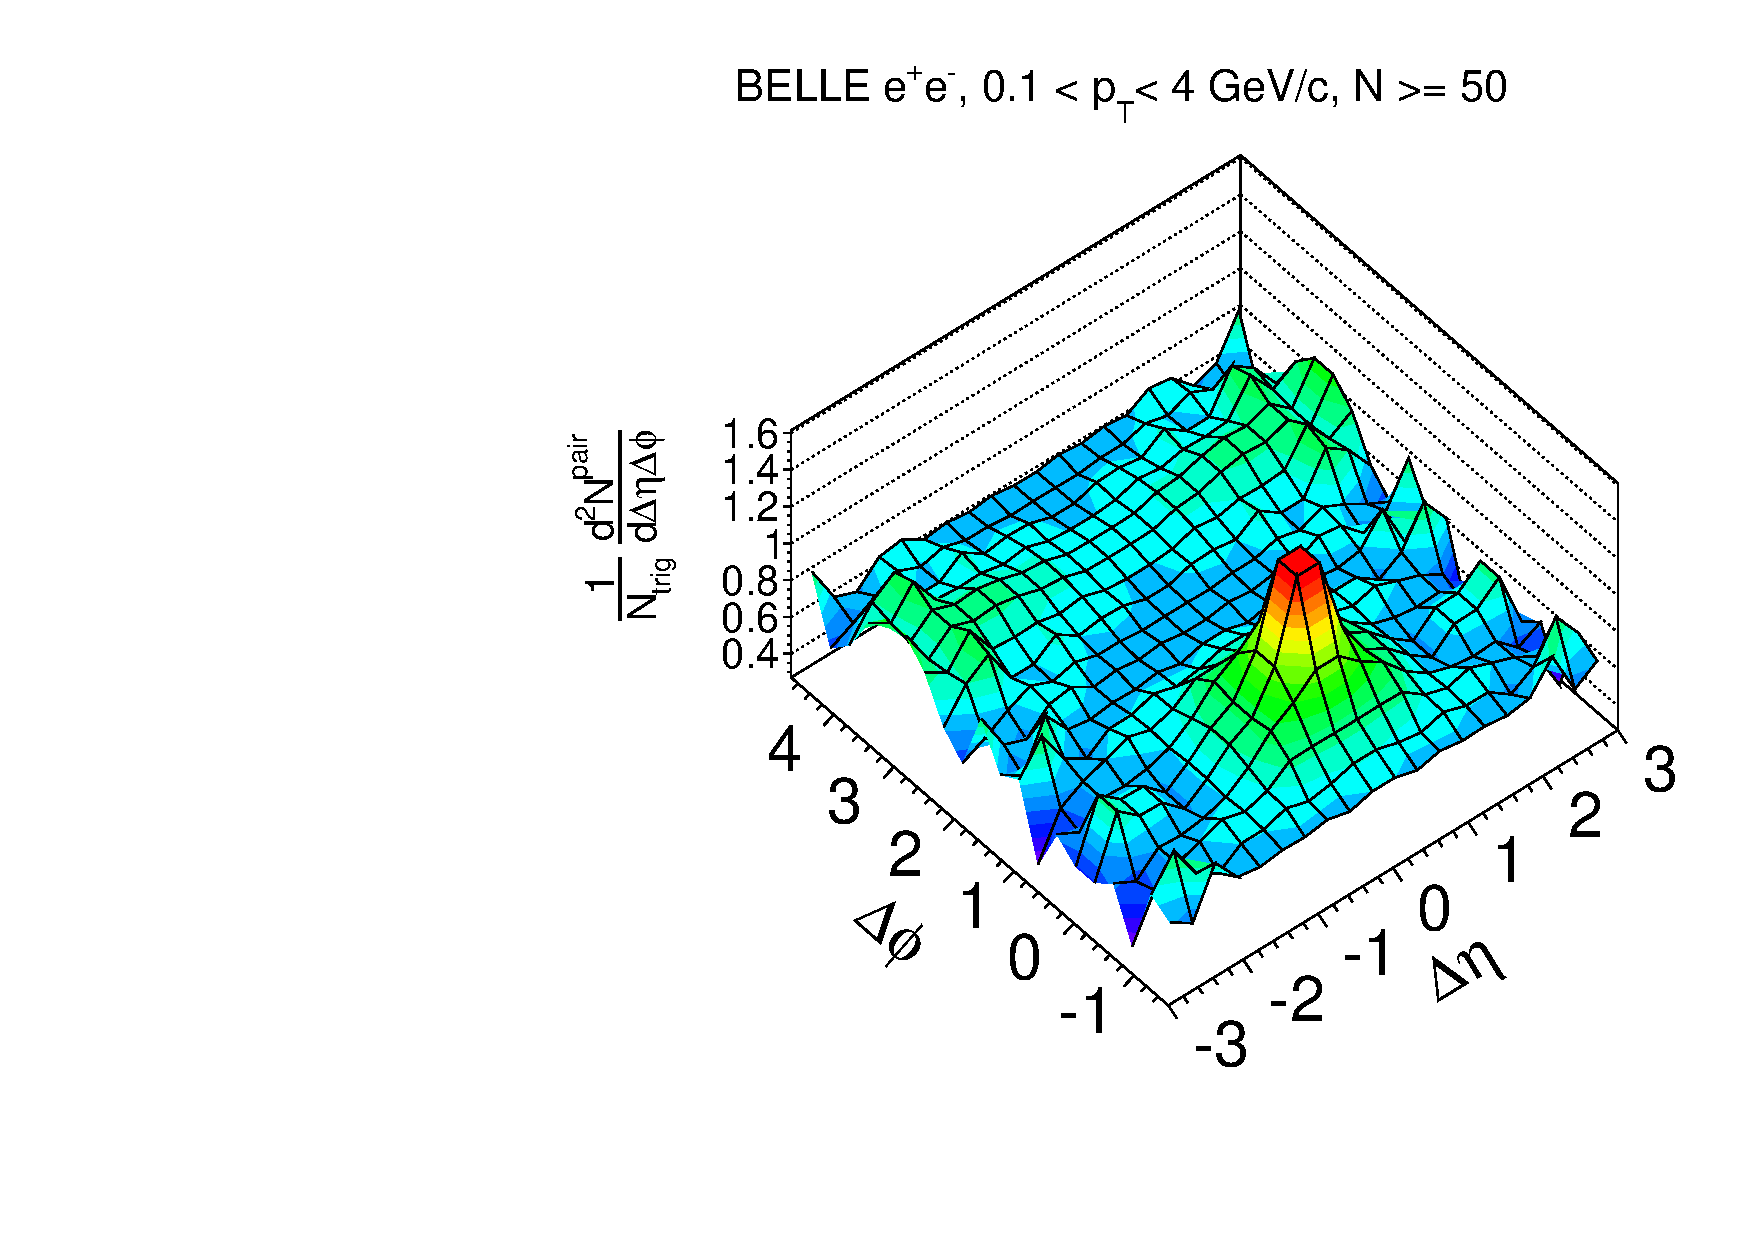
\includegraphics[width=.45\textwidth]{figures/canvasRidgeBelleMult50CutHigh0.pdf}
\caption{Two-particle correlation functions versus $\Delta\eta$ and $\Delta\phi$ in $e^{+}e^{-}$ collisions for events with particle multiplicity $>$ 20 (top left), 40 (top right), 50 (bottom).}
\label{fig:ridgeBelle} 
\end{center}
\end{figure}


\begin{figure}[!htb]
\begin{center}
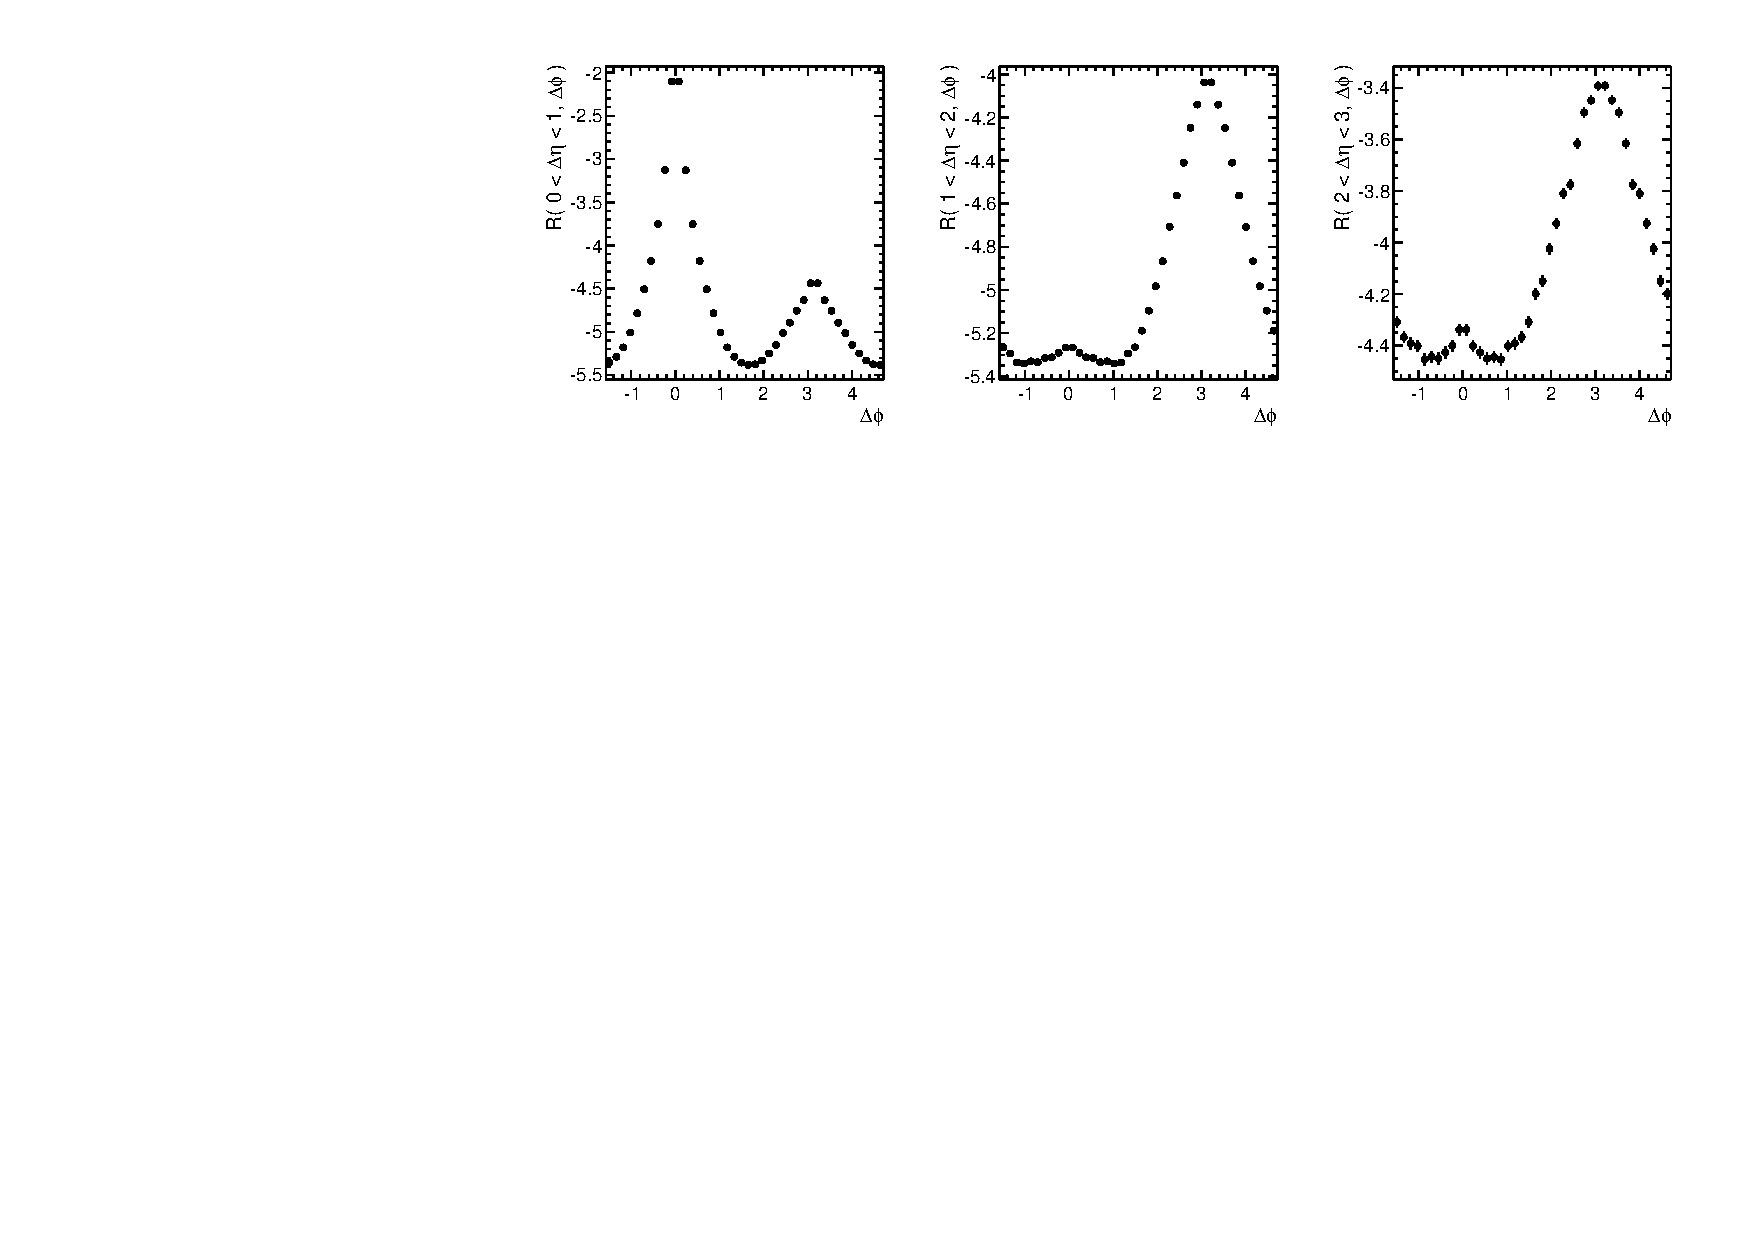
\includegraphics[width=.95\textwidth]{figures/canvasProjection_isBelle1_mult20.pdf}
\caption{$\rm \Delta R$ ($\rm \Delta\phi$) for events with total multiplicity N$>=$ 20. }
\label{fig:ProjectionMult20} 
\end{center}
\end{figure}

\begin{figure}[!htb]
\begin{center}
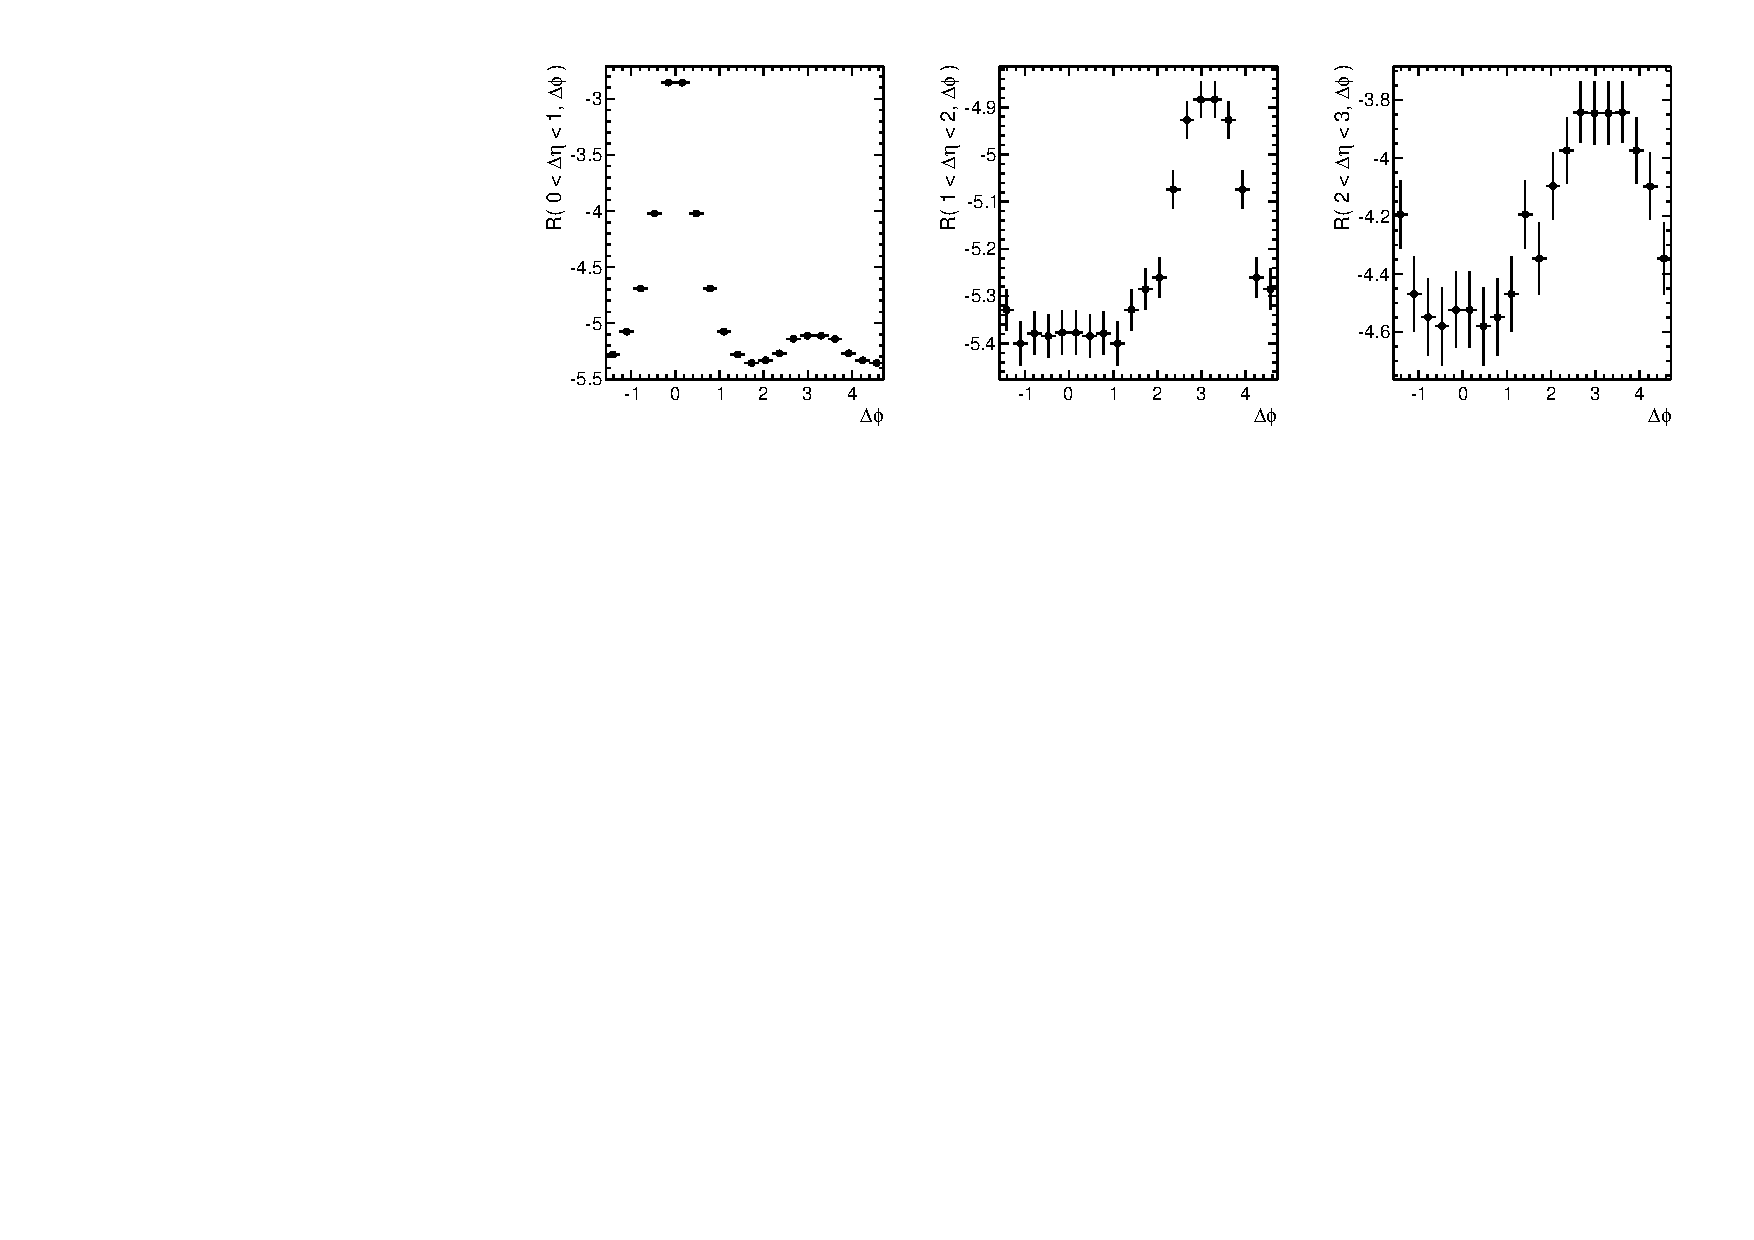
\includegraphics[width=.95\textwidth]{figures/canvasProjection_isBelle1_mult40.pdf}
\caption{$\rm \Delta R$ ($\rm \Delta\phi$) for events with total multiplicity N$>=$ 40. }
\label{fig:ProjectionMult40} 
\end{center}
\end{figure}

\begin{figure}[!htb]
\begin{center}
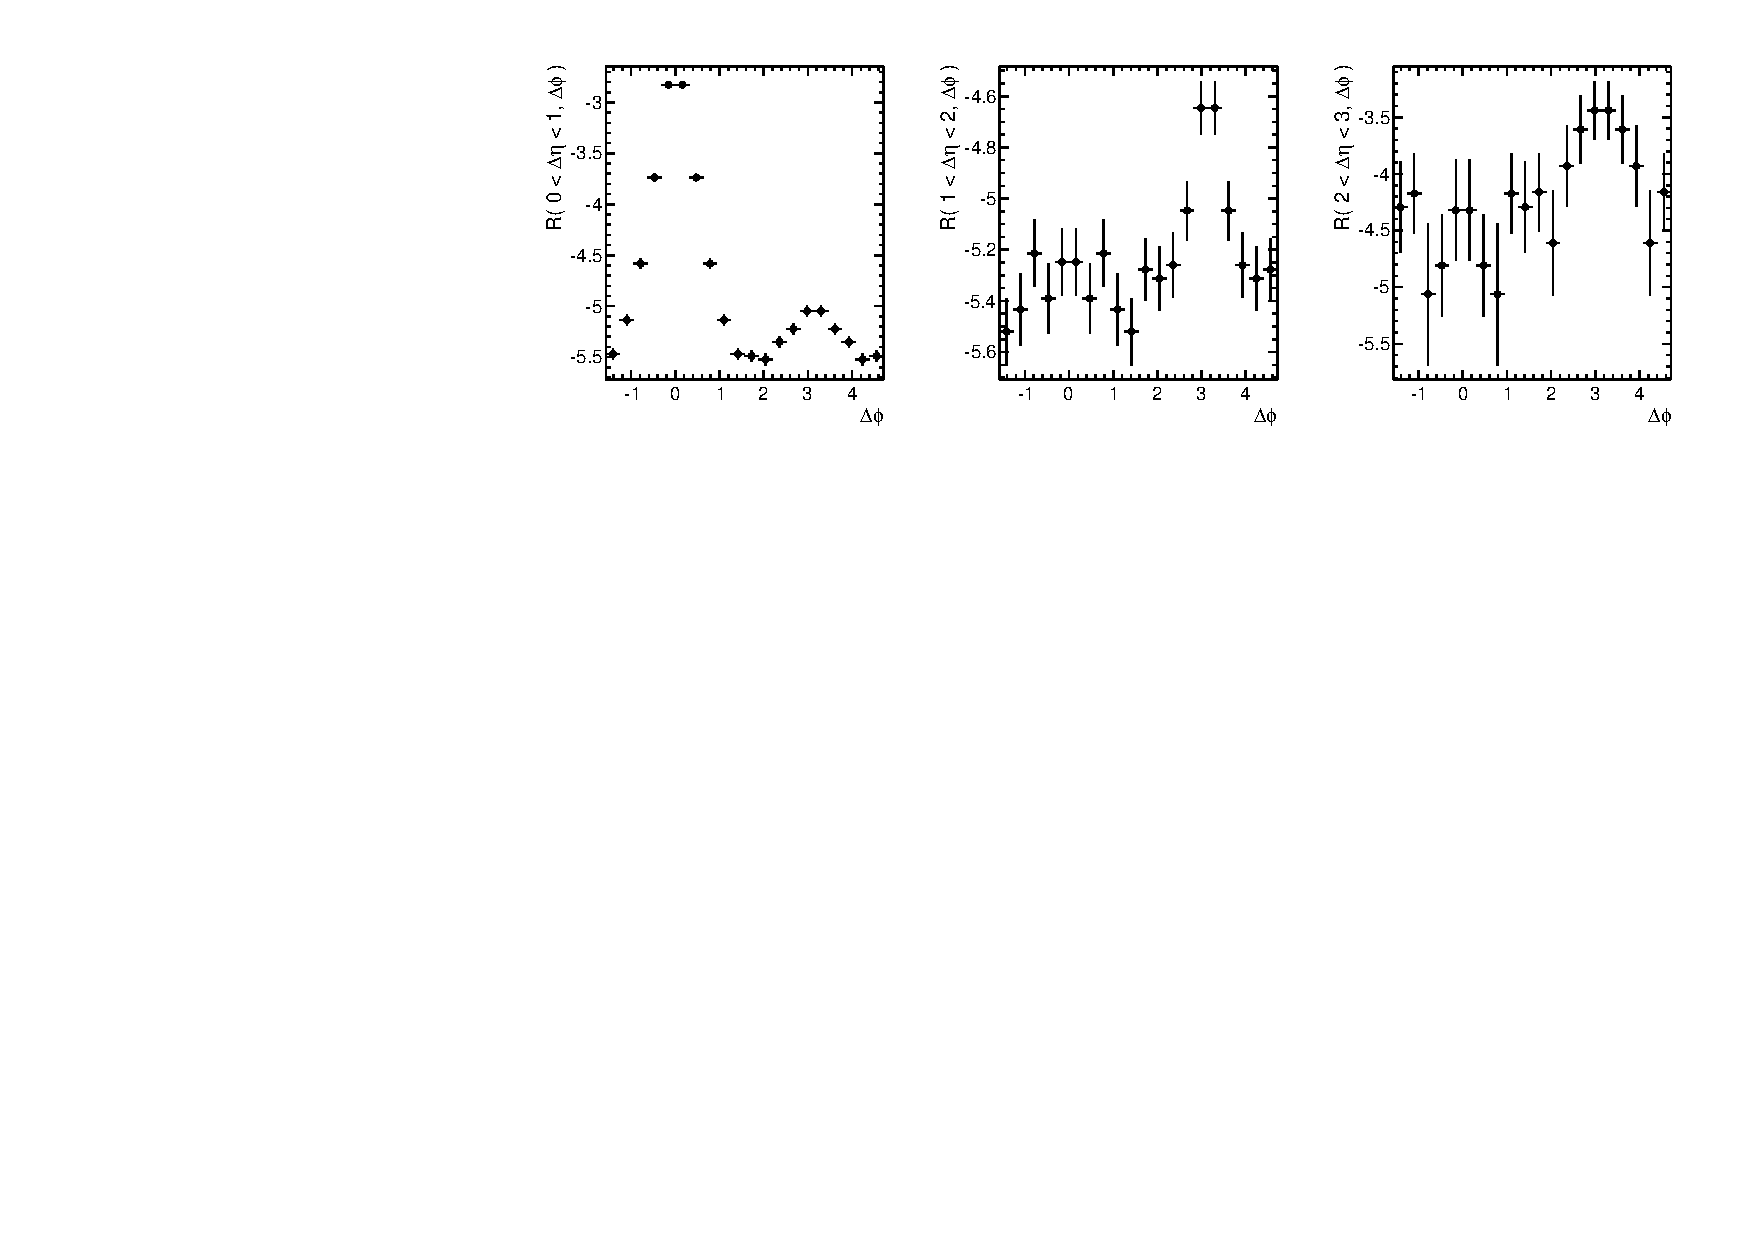
\includegraphics[width=.95\textwidth]{figures/canvasProjection_isBelle1_mult50.pdf}
\caption{$\rm \Delta R$ ($\rm \Delta\phi$) for events with total multiplicity N$>=$ 50. }
\label{fig:ProjectionMult50} 
\end{center}
\end{figure}


\end{document}
%
% ****** End of file apssamp.tex ******
